\documentclass[xcolor=dvipsnames,t]{beamer} % position stuff on top of slide
% Functions, packages, etc.
%[[[
\usetheme{Frankfurt}
\usecolortheme[named=Maroon]{structure}

% Remove Navigation Symbols
\usenavigationsymbolstemplate{}

\usepackage{amsmath}
\usepackage{amsfonts}
\usepackage{amssymb}
\usepackage{array}

\usepackage{tikz}

\usepackage{graphicx}
\usepackage{subfig}
\usepackage[labelfont=bf]{caption}
\captionsetup{font=small}
\usepackage{hyperref}

\newcommand{\diff}[2]{\dfrac{d #1}{d #2}}
\newcommand{\diffn}[3]{\dfrac{d^{#3} #1}{d {#2}^{#3}}}
\newcommand{\pdiff}[2]{\dfrac{\partial #1}{\partial #2}}
\newcommand{\pdiffn}[3]{\dfrac{\partial^{#3} #1}{\partial {#2}^{#3}}}
\newcommand{\problemline}{\rule{\textwidth}{0.25mm}}
%\newcommand{\problem}[1]{\problemline\\#1\\\problemline\vspace{10pt}}
\newcommand{\reals}{\mathbb{R}}
\newcommand{\qline}[2]{\qbezier(#1)(#1)(#2)}
\newcommand{\abox}[1]{\begin{center}\fbox{#1}\end{center}}
%]]]

% Output Control Variables
\def\true{1}
\def\false{0}
\def\figures{1}
\def\tables{1}

\renewcommand{\UrlFont}{\scriptsize}
\newcommand{\defeq}{\mathrel{\mathop:}=}

% beamer description align left template
% http://tex.stackexchange.com/questions/95964/right-description-list-latex-beamer
\defbeamertemplate{description item}{align left}{\insertdescriptionitem\hfill}


\title{Automated Music Genre Classification}
\date{3 December, 2014}
\author{James Folberth, Aly Fox, Dale Jennings}

\begin{document}

\begin{frame}
\maketitle
\end{frame}

% TODO: these items are in no particular order and might not have the best names.  Please rename them and move them around as you wish.  Make sure that the section names match the names in the outline

\begin{frame}{Outline}
   %Outline:
   \setbeamertemplate{description item}[align left] % align left
   \begin{description}                              % align left
   %\setbeamertemplate{description item}[default]  % align right
   %\begin{description}[Clustering/Classification] % align right
      \item[Features] Spectral, Temporal, Wavelet Coefficient Histograms\\
      \item[Dimension Reduction] PCA, LLE, PageRank, Graph Laplacian\\
      \item[Clustering/Classification] kNN, SVM with multi-class, Graph Laplacian\\
      \item[Discussion]
   \end{description}

\end{frame}



\section{Features}
\begin{frame}{Mel Frequency Cepstral Coefficients}
   Dale, I guess.  Talk about what we're doing in the Fourier power, Mel power, temporal domains

\end{frame}

% James
\begin{frame}{Wavelet Coefficient Histograms}
   \begin{columns}[T,onlytextwidth]
      \begin{column}{0.45\textwidth}
         \begin{itemize}
            \item The wavelet transform generally has good time and frequency resolution.
            \item Complex temporal signals become more simple in the wavelet domain.
            \item We look at the histogram of wavelet coefficients in each sub-band.
         \end{itemize}

      \end{column}

      \begin{column}{0.45\textwidth}
         The multiresolution idea:\\[1em]
         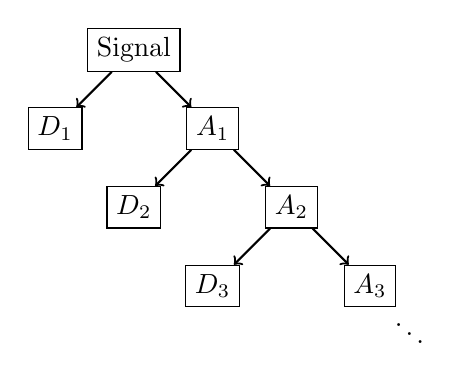
\begin{tikzpicture}
            \node[draw] (signal) at (0,0) {Signal};
            \node[draw] (a1) at (1,-1) {$A_1$};
            \node[draw] (d1) at (-1,-1) {$D_1$};

            \node[draw] (a2) at (2,-2) {$A_2$};
            \node[draw] (d2) at (0,-2) {$D_2$};

            \node[draw] (a3) at (3,-3) {$A_3$};
            \node[draw] (d3) at (1,-3) {$D_3$};

            \node (etc) at (3.5,-3.5) {$\ddots$};

            \draw[thick,->] (signal) -- (a1);
            \draw[thick,->] (signal) -- (d1);
            \draw[thick,->] (a1) -- (a2);
            \draw[thick,->] (a1) -- (d2);
            \draw[thick,->] (a2) -- (a3);
            \draw[thick,->] (a2) -- (d3);

         \end{tikzpicture}
      \end{column}
   \end{columns}
\end{frame}

% James
\begin{frame}{Wavelet Coefficient Histograms}
   Idea: The WCHs are characterized by their moments.

   The WCH features are extracted as follows:
   \begin{enumerate}
      \item Compute the wavelet decomposition of the central $~23$ seconds.
      \item Construct the histogram for each sub-band.
      \item Compute the first three moments of each histogram (mean, variance, skewness).
      \item Compute a sub-band energy for each histogram.
   \end{enumerate}

   % Not all subbands contain useful information
\end{frame}

% James
\begin{frame}{Wavelet Coefficient Histograms}
   Features from detail sub-bands $4,5,6,7$:\\

   ~\\[-10em]
   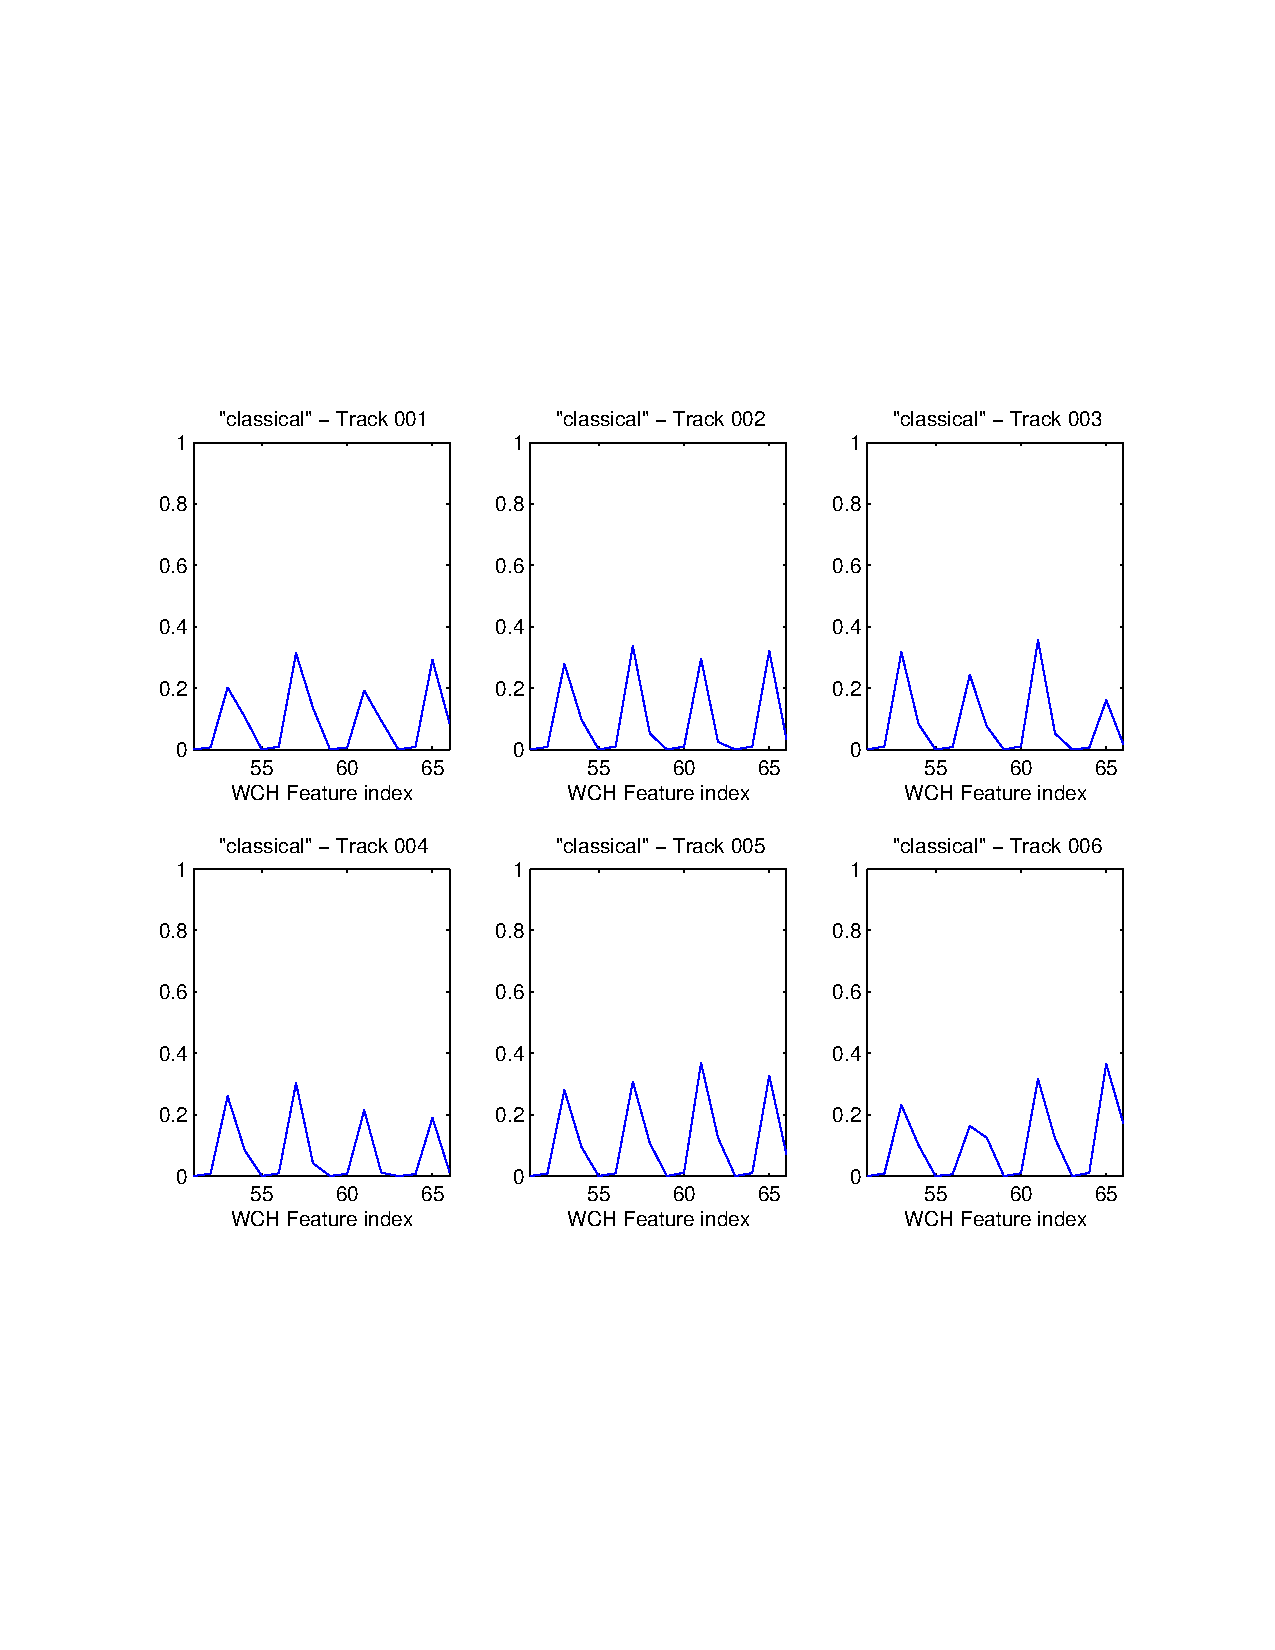
\includegraphics[width=\textwidth]{figures/wch_class.pdf}

\end{frame}

% James
\begin{frame}{Wavelet Coefficient Histograms}
   Features from detail sub-bands $4,5,6,7$:\\

   ~\\[-10em]
   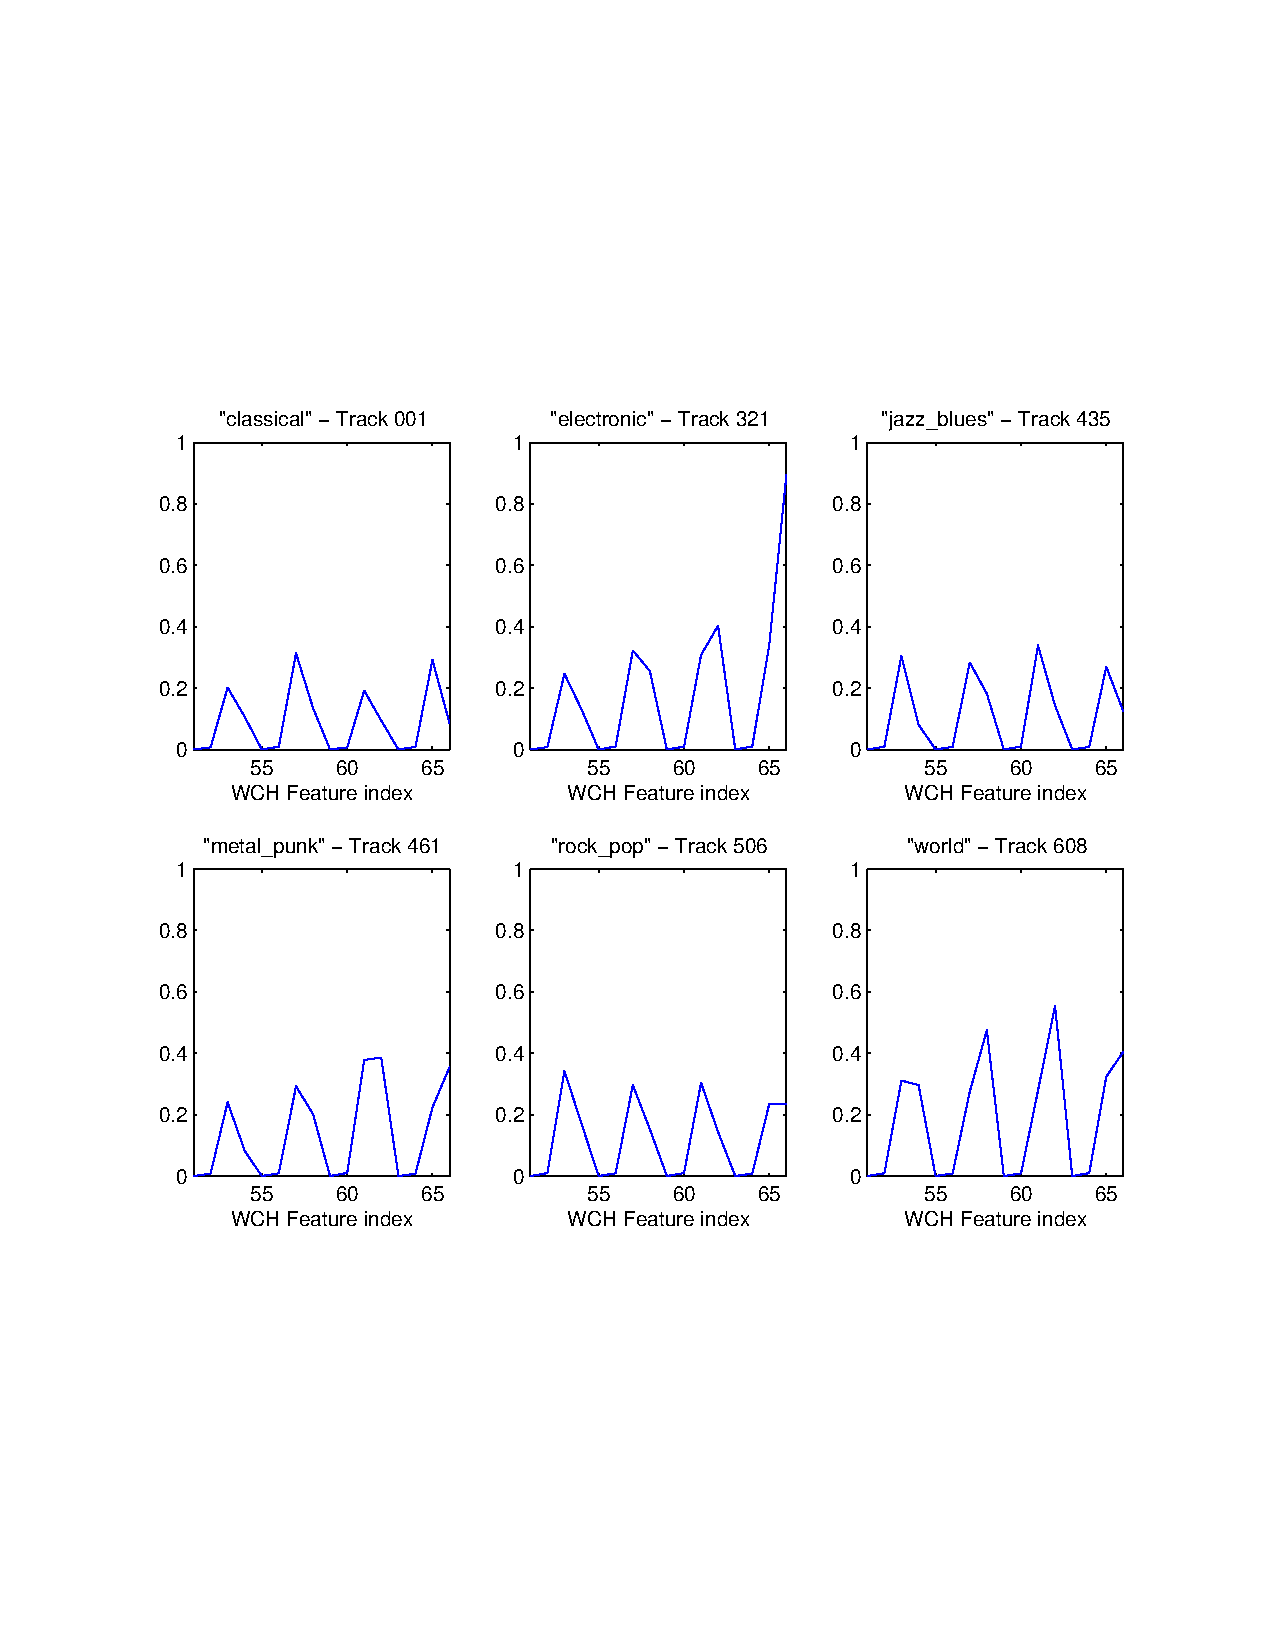
\includegraphics[width=\textwidth]{figures/wch_diff.pdf}

\end{frame}

% James
% Stolen from Li et al. SIGIR 2003
%\begin{frame}{Wavelet Coefficient Histograms}
%   \begin{columns}[T,onlytextwidth]
%      \begin{column}{0.25\textwidth}
%         From Li et al., \emph{SIGIR} '03.\\
%      \end{column}
%
%      \begin{column}{0.7\textwidth}
%         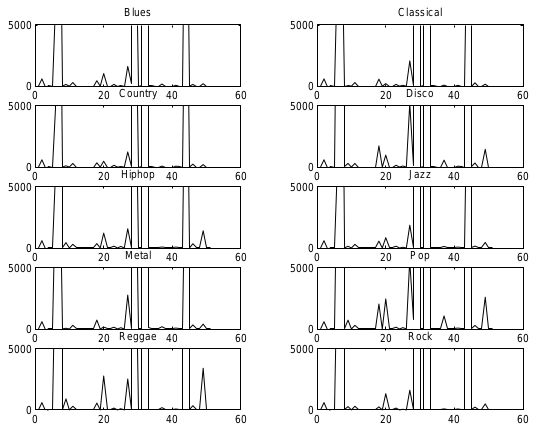
\includegraphics[width=\textwidth]{figures/wch_li_1.png}
%      \end{column}
%   \end{columns}
%\end{frame}


\section{Dimension Reduction}
\begin{frame}{PCA with $k$-Nearest Neighbors classifier}
Optimization of parameters for Dale + WCH

PCA tends to mess up 
\end{frame}

\begin{frame}{LLE with $k$-Nearest Neighbors classifier}
Optimization of parameters for Dale + WCH
\end{frame}

\begin{frame}{Super awesome PageRank feature selection}
Dale
\end{frame}

\begin{frame}{Graph Laplacian}
Aly
\end{frame}



\section{Clustering/Classification}
\begin{frame}{SVM classifiers}
Describe linear SVM.\\
Use kernel trick (with soft margin).\\
We use polynomial kernel with varying order $p$:

\[ k(\mathbf{x}_i,\mathbf{x}_j) = \left(1 + \mathbf{x}_i\cdot\mathbf{x}_j\right)^p. \] 

% TODO Try Gaussian again
\end{frame}
%\begin{frame}{PCA/LLE + SVM classifiers}
%James
%\end{frame}

\begin{frame}{Graph Methods}
Aly
\end{frame}


\section{Discussion}

\begin{frame}{References}
   \begin{itemize}
      \item G. Sussman and J. Wisdom, \emph{Numerical evidence that the motion of pluto is chaotic}, Science, (1988).\\
      \item J. Wisdom and M. Holman, \emph{Symplectic maps for the n-body problem}, The Astronomical Journal, (1991).\\
   \end{itemize}
   ~\\
   Questions?

\end{frame}

\end{document}

% vim: set spell:
% vim: foldmarker=[[[,]]]
